\documentclass[]{llncs}
\usepackage[T1]{fontenc}
\usepackage[utf8]{inputenc}
\usepackage{url}
\usepackage{comment}
\usepackage{graphicx}
\usepackage{multirow}
\usepackage{booktabs}
\usepackage{amsmath}
\usepackage{scalefnt}

\usepackage{tikz}
\usetikzlibrary{fit}

\usepackage{acronym}
\acrodef{iaas}[IaaS]{Infrastructure as a Service}
\acrodef{SaaS}{Software as a Service}
\acrodef{PaaS}{Platform as a Service}
\acrodef{dag}[DAG]{directed acyclic graph}
\acrodef{vm}[VM]{Virtual Machine}
\acrodef{pm}[PM]{Physical Machine}
\acrodef{btu}[BTU]{billing time unit}
\acrodef{EC2CU}{EC2 Compute Unit}
\acrodef{HPC}{High Performance Computing}
\acrodef{unistra}{University of Strasbourg}
\acrodef{rv}[RV]{random variable}
\acrodef{pdf}[PDF]{probability density function}
\acrodef{cdf}[CDF]{cumulative distribution function}
\acrodef{mcs}[MCS]{Monte-Carlo simulation}
\acrodefplural{mcs}[MCS's]{Monte-Carlo simulations}
\acrodef{des}[DES]{discrete event simulation}
\acrodef{ci}[CI]{confidence interval}

\newcommand*\rot{\rotatebox{90}}
\newcommand{\pmpc}[1]{$\pm#1\%$}
\newcommand{\etal}[1]{\emph{#1 et al.}}
\newcommand{\pc}[1]{$#1\%$}


%\IEEEtriggeratref{15}

%\title{Modeling the accuracy of Monte-Carlo approach for Cloud based workflow
%  simulations.}
%\title{Executing Batch Jobs on Clouds: How to Predict Reality Accurately?}
\title{Improving Cloud Simulation using the Monte-Carlo Method}


\author{Luke~Bertot
	\and Stéphane~Genaud 
	\and Julien~Gossa}
\institute{Icube-ICPS --- UMR 7357, Univeristé de Strasbourg, CNRS\\
		P\^ole API Blvd S. Bant, 67400 Illkirch%\\
	%	email: \url{lbertot@unistra.fr}, \url{genaud@unistra.fr}, \url{gossa@unistra.fr}
	}



\begin{document}

\maketitle

\begin{abstract}
  In the  cloud computing  model, cloud providers  invoice clients  for resource
  consumption. Hence, tools helping the client to budget the cost of running his
  application are  of pre-eminent  importance. However, the opaque and 
  multi-tenant nature of clouds make task runtimes variable and hard to predict,
  and hamper the creation of reliable simulation tools. In this  paper, we 
  propose an improved simulation framework that takes into account this 
  variability using the Monte-Carlo method.

  We consider  the execution of  batch jobs on an actual platform, scheduled
  using typical  heuristics based on the user estimates  of task  runtimes.  We
  model  the observed  variability through  simple  random variables  to use  as
  inputs  to the  Monte-Carlo  simulation.  Based  on  this stochastic  process,
  predictions are expressed as interval-based  makespan and cost.  We show that,
  our method  can capture over  90\% of  the empirical observations  of makespan
  while keeping the capture interval size below 5\% of the average makespan.
\end{abstract}


%\tableofcontents

\section{Introduction}

Over the  last decade, the advancement  of virtualization techniques has  led to
the emergence of new economic  and exploitation approaches of computer resources
in  \ac{iaas}, one  form  of  cloud computing.   In  this  model, all  computing
resources are made  available on demand by third-party operators  and paid based
on usage.  The  ability to provision resources  on demand is mainly  used in two
ways.  First, it  can serve for scaling purposes where  new machines are brought
online to face higher workloads and allows for a lower baseline cost.
Secondly, it  is useful  for parallelizing tasks to  achieve a  shorter makespan
(\textit{i.e.}\  the time  between  the  submission of  the  first task and  the
completion of the  last task) at equal  cost, this approach being  often used for
scientific  and  industrial  workloads  when runtime  is  heavily  dependent  on
computing power.  This  approach is made possible by the  pricing model of cloud
infrastructures, as  popularized by Amazon Web Services, in which
payment  for computing  power provided  as \acp{vm},  happens in  increments of
arbitrary lengths of  time, \ac{btu}, usually of one hour. % Running two \acp{vm}
%side by side  for one \acp{btu} actually  costs the same as  running one \ac{vm}
%for two \acp{btu}, but every \ac{btu} started is owed in full.
%
This model  offers the client  an almost complete freedom  to start or  stop new
servers as long as it can be afforded. However, for distributed applications, it
quickly becomes  difficult to manually  provision the resources in  an efficient
way.  The  use of a scheduler  becomes unavoidable for such  workloads.  In this
paper,  we are  interested in  predicting the  execution time  and cost  of such
workloads, in which  the scheduling plays an important role. 

%----------------------- prediction tools --------------------------------------
Independently  of  scheduling  decisions,  the accurate  prediction  of  complex
workload execution is hampered by  the inherent variability of clouds, explained
by multiple factors.  First \ac{iaas} operates  in an opaque fashion~: the exact
nature of the underlying platforms is unknown, and their hardware are subject to
evolution.   Secondly  cloud systems  are  multi-tenant  by nature.   This  adds
uncertainty due to contention on network and memory accesses.  This variability,
reported  by  a  number  of practitionners  who  evaluate  parallel  application
performance  on  clouds  (e.g~\cite{MehrotraDHHJLSB16}, who  report  an  average
5\%-6\% variability on AWS cluster compute instances), has also been measured by
one   of   the   most   comprehensive   and  recent   survey   by   Leitner   et
al.~\cite{LeitnerC16}.  We will see in this paper that our observations fit with
the figures presented in this survey.
%
This  variability increases  the difficulty  of modeling task execution  times.
%which is  already difficult  enough, as  shown in~\cite{Lastovetsky05}.  
In this regard,  the prediction is highly dependent on  the underlying simulator
of the system and on the phenomena it can capture.  In this work, we rely on the
SimGrid~\cite{simgrid} simulation  toolkit, enabling us to  build discrete event
simulators of distributed systems such as Grids, Clouds, or HPC systems. SimGrid
has   been    chosen   for    its   well-studied   accuracy    against   reality
(e.g.~\cite{StanisicTLVM15,VelhoSCL13}).    In  particular,   given  a   precise
description  of the  hardware platform,  its  network model  takes into  account
network contention in presence of multiple communication flows.

However, we may not be able to provide a fully accurate platform description, or
be unable to  estimate the network cross-traffic, yielding  a distortion between
simulation and reality.  To deal with  this problem, the standard approach is to
consider task runtimes to be stochastic. Every  task can be modeled by a \ac{rv}
that models  the whole  spectrum of  possible runtimes.  These \acp{rv}  are the
basis required for a stochastic simulation.  Such simulations output \acp{rv} of
the observed phenomenon  (\emph{makespan} or \emph{\ac{btu}}) which  in turn can
be used to create intervals of possible results with their assorted confidence.
%
In this paper, we propose a stochastic method to enrich the classical prediction
based  on the  discrete-event simulator  SimGrid,  and we  study the  conditions
needed for  this approach to be  relevant. This study  is carried out in  a real
setting,  described in  section~\ref{sec:work-context},  where the  applications
use-cases, the scheduler, and the  experimental observations are presented.  The
stochastic     framework     we     propose     is     then     presented     in
section~\ref{sec:enriched-sim}  and is  evaluated in  section~\ref{sec:eval}. %We
%finally conclude by  discussing in section~\ref{sec:disc} the possible
%improvements and the  limits of the approach.


\section{Related Work}
\label{sec:relworks}

%Because they allow  for experiments without having  to build or even  use a real
%platform, simulations are a cornerstone of  the study of distributed systems and
%clouds.
\paragraph{Simulation.} Most cloud simulators  are based on \ac{des}. In \aclp{des}  the simulation is a
serie  of events  changing the  state of  the simulated  system.  For  instance,
events can  be the  start (or  end) of computations  or of  communications.  The
simulator will jump from  one event to the next, updating  the times of upcoming
events  to reflect  the state  change  in the  simulation.  Such  \ac{des}-based
simulators  require  at  least  a  platform  specification  and  an  application
description.  %The platform  specification describes both the  physical nature of
%the cloud,  e.g.~machines and networks,  and the management  rules, e.g.~\ac{vm}
%placement  and   availability.   
%Depending on the simulator, the platform  specification can be done through user
%code,  as   in  CloudSim~\cite{cloudsim}   for  example,  or   through  platform
%description  files,  as  is  mostly the  case  in  SimGrid~\cite{simgrid}.   The
%application description consists in a  set of computing and communicating tasks,
%often described  as an amount  of computation  or communication to  perform. The
%simulator computes their  duration based on the platform  specification, and its
%CPU and network models.  %An alternative approach
%is  to directly  input the task  durations extrapolated  from actual  execution
%traces.
%
The available  cloud \acp{des} can  be divided in  two categories. In  the first
category are  the simulators  dedicated to  study the  clouds from  the provider
point-of-view, whose purpose  is to help evaluating the design  decisions of the
datacenter. 
% ---
Examples  of such simulators are  MDCSim~\cite{MDCSim}, which offers
specific  and precise  models for  low-level components  including network  (e.g
InfiniBand or  Gigabit ethernet),  operating system kernel  and disks.   It also
offers a model  for energy consumption. However, the cloud  client activity that
can be  modeled is restricted  to web-servers, application-servers  or data-base
applications.   GreenCloud~\cite{greencloud} follows  the  same  purpose with  a
string  focus  on  energy  consumption  of cloud's  network  apparatus  using  a
packet-level  simulation  for  network  communications  (NS2).   
% ---
In the  second category  (which we  focus on) are  the simulators  targeting the
whole   cloud  ecosystem   including  client   activity.   In   this  category,
CloudSim~\cite{cloudsim}  is  the  most   broadly  used  simulator  in  academic
research.  It offers simplified models  regarding network communications, CPU or
disks. However, it is easily extensible  and serves as the underlying simulation
engine in a number of projects. Simgrid~\cite{simgrid} is the other long-standing
project,  which  when used  in  conjunction  with  the SchIaaS  cloud  interface
provides  similar  functionnalities  as   CloudSim.   Among  the  other  related
projects, are iCanCloud~\cite{iCanCloud} proposed  to address scalability issues
encountered  with  CloudSim  (written  in  Java) for  the  simulation  of  large
use-cases.  Most recently,  PICS~\cite{pics} has  been proposed  to specifically
evaluate simulation of  public clouds.  The configuration of  the simulator uses
only parameters  that can be  measured by the  cloud client, namely  inbound and
outbound  network  bandwidths,  average  CPU  power,  \ac{vm}  boot  times,  and
scale-in/scale-out policies. The  data center is therefore seen as  a black box,
for which  no detailed  description of  the hardware  setting is  required.  The
validation study  of PICS  under a  variety of use  cases has  nonetheless shown
accurate predictions.

%At the core of DES is the solver.  The solver considers the states of the system
%generated  by the  platform and  previous events  to compute  the timing  of the
%future events. 
%In  most  cases, simulators  have  a  \emph{bottom-up} approach~:  the  modeling
%concerns low-level  components (machines,  networks, storage devices),  and from
%their interactions  emerge the high-level  behaviours. Working on  disjoint low
%level components make it easier to tune the precision of the model to the wanted
%accuracy or speed trade-off.

However, when the simulated system is subject to variability, it is difficult to
establish  the  validity of  simulation  results  formally. Indeed,  given  some
defined inputs, a DES outputs a single deterministic result, while a real system
will output  slightly different results  at each repeated execution.   Hence, in
practice  the simulation  is informally  regarded as  valid if  its results  are
``close'' to one or  some of the real observations. 
%Notice  however that in the
%field  of grid  or cloud  computing, published  results in  terms of  validation
%against real settings are scarce relatively to the number of projects.

\paragraph{Stochastic Simulation and Monte-Carlo Method.}
For  more   comprehensive  predictions  in  such   variable  environments,  the
simulation must  be \emph{stochastic}.  In stochastic simulations  inputs become
\acfp{rv} representing the  distribution of possible values  for the parameters.
The  result  of one  such  simulation  is  itself  an \ac{rv}  representing  the
distribution  of the  results. 

Extensive  work  has  been  done  on numerical  methods  for  solving  stochastic
simulations of  \ac{dag}~\cite{Li97,Ludwig01}. In a \ac{dag}  model the vertices
represent  the tasks  comprising the  application, and  the edges  represent the
dependencies   between   those   tasks.   The   numerical   approach   presented
in~\cite{Li97,Ludwig01}  shows that,  when tasks'  runtimes are  independent, the
makespan distribution of two successive tasks  is the convolution product of the
tasks'  \aclp{pdf}, while  the makespan  of two  parallel tasks  joining is  the
product  of   the  tasks'   \aclp{cdf}.  This   makes  the   numerical  approach
computationally  intensive   and  its  core  constraint,   the  tasks  \acp{rv}
independence, can  not be guaranteed  in all cases. Moreover  this \ac{dag}-based
approach  implies  fixed  scheduling,  since  the  scheduling  creates  implicit
dependencies between tasks scheduled one after another. In a cloud context where
resources can be provisioned on the fly, dynamic scheduling is much more common.

Instead of numerically computing the  resulting \ac{rv}, a \ac{mcs} samples the
possible  results by  testing  multiple \emph{realizations}  in a  deterministic
fashion.  A  realization is  obtained by  drawing a  runtime that  follows their
task's respective  \ac{rv} for every  task in  the application.  This  allows to
simulate each realization using  traditional methods like \ac{des}.  Eventually,
given enough realizations, the distribution  of the simulation results will tend
towards the  distribution of the equivalent  stochastic simulation.  Statistical
fitting   techniques  can   then   be  used   to   characterize  this   makespan
\ac{rv}. \acp{mcs} allows for non-independent \ac{rv} and dynamic
scheduling.
This approach is first suggested in
\cite{Slyke63}  for stochastic  PERT graphs.   
%The development  of heterogeneous
%distributed computing environments, grids and now clouds, has led researchers to
%se this approach in  this field.  
Later, in the  context of grids, where  the number of resources  is fixed during
one execution, Tang et al.~\cite{Tang11} propose, a modification of the well-known
scheduling heuristic HEFT to compute a schedule yielding the shortest makespan
given randomly variable task durations. Canon and Jeannot~\cite{Canon10} have
used \ac{mcs} to evaluate the robustness of \ac{dag}
schedules when task  durations vary, and similarly,  Zheng et al.~\cite{Zheng13}
evaluate  the  impact of  this  variability  on  the makespan.   More  recently,
ElasticSim~\cite{Cai17} has been  proposed as a simulator  extending Cloudsim to
integrate resource auto-scaling and stochastic  task durations. Similarly to our
work, ElasticSim computes a schedule whose  objective is to minimize rental cost
while meeting deadline constraints.  For  several generated workflows, the study
compares the simulation results regarding rental cost and makespan, when varying
the  variability  of task  duration  and  deadline  with arbitrary  values.   By
contrast,  our  work focuses  on  how  the  \ac{mcs}  method, under  some  given
variability assumptions, captures actual observations.


\section{Work Context}
\label{sec:work-context}

The study  conducted in this  paper is built  upon a genuine  comparison between
experiments  run in  actual environments  and experimental  results obtained  by
simulation.   To strengthen  the validity  of the  comparison, the  experimental
conditions  for  the  real  setup  and  the  simulation  should  share  as  many
commonalities as possible, as advocated in~\cite{PucherGWK15}.  Our experimental
setup described hereafter consists of two test applications which are on one
hand, run on a real platform with our scheduler Schlouder, and on the other hand are
simulated with our simulator SimSchlouder based on SimGrid.

\paragraph{Test Applications}\label{sc:setup}

We  carried out  multiple executions  of two broadly used scientific  applications
to  evaluate Schlouder  performance. The execution traces for  those runs were
collected  in an  archive.  This backlog  of real  executions  is the  benchmark
against which  our simulation  performance will  be evaluated.  Those applications
are:

\begin{itemize}
\item Montage\cite{montage2009},  the Montage Astronomical Image  Mosaic Engine,
  is designed to  splice astronomical images. This application is a data
  intensive fork-join type workflow with a \emph{communication-to-computation} 
  ratio greater than $90\%$.

\item OMSSA\cite{Geer2004}, the Open Mass-Spectrometry Search Algorithm, is used
  to analyze  mass-spectrometer results.  The application  is a computation
  intensive set of independent parallel tasks  with a 
  \emph{communication-to-computation} ratio lower than $20\%$.
\end{itemize}

\paragraph{Real Execution Setup}
Schlouder~\cite{Michon17} is a client-side cloud broker for IaaS capable of
executing the  user's batch jobs, sets of independent tasks and workflows alike.
The broker's main role is  to schedule the tasks onto a set of cloud resources, 
which the broker can scale up  or down.
Technically, the broker  connects to the cloud management  system (for instance,
OpenStack) to  instruct how  the infrastructure should  be provisioned. It then
assigns the tasks to the resources using the Slurm job management system.
%
As in  most batch scheduler systems,  the task description includes  its runtime
estimation by the user called \emph{user  estimate}.  In case of a workflow, the
task  dependencies are  also provided.   Schlouder uses  just-in-time scheduling
where  tasks are  assigned to  \acp{vm} as  soon as  all their  dependencies are
satisfied.  A  task's real  runtime,  called  \emph{effective runtime},  usually
differs from  estimated runtimes, but  this does not change  previous scheduling
decisions. Schlouder's scheduling and provisioning  decisions are controlled by a
\emph{strategy}.  These strategies  are  bi-objective, taking  into account  the
rental cost of resources and the execution  makespan. In this paper, we used the
two following strategies :
\begin{itemize}
\item ASAP (\textit{as soon as possible}) schedules each task onto
  an idle VM if one is available, or provisions a new VM otherwise.
  This strategy minimizes the makespan.

\item AFAP (\textit{as full as  possible}) schedules each task onto
  one VM if it does not increase the rental cost (\textit{i.e.} the number
  of \ac{btu}), or provisions a new VM otherwise. This strategy minimizes cost
  by minimizing the \ac{btu} count.
\end{itemize}

\paragraph{Simulated Execution Setup.}
As a follow-up to our work on Schlouder we developed SimSchlouder, a simulator
mimicking the behaviour of Schlouder. It has the same interfaces and implements
the same scheduling strategies as Schlouder. It uses SimGrid as its core
simulation engine. In practice, SimSchlouder is included as a plugin into
Schlouder to allow the user to request an estimate of the makespan and cost
before choosing a strategy for a real run.
%
SimSchlouder  shares with Schlouder a common subset of inputs, including
the same tasks description and strategy. Whereas Schlouder operates on a
real cloud controller, SimSchlouder provisions simulated \acp{vm} through
SimGrid's cloud interface called SchIaaS. Additionally SimSchlouder requires a
platform specification, which describe the physical nature of the cloud as well
as the management rules, and the effective runtime of each task, that are used
by the simulator to compute the tasks' end dates. Together, they allow the
simulation to be accurately representative of reality.

\section{Proposal: an Enriched Simulation Framework}\label{sec:enriched-sim}


To address the limited trustworthiness of \ac{des} in variable environments such
as clouds, we propose a framework implementing the Monte-Carlo method using 
SimSchlouder as simulation engine. This  solution combines the extensive results
provided  by stochastic simulations with correctness of scheduling and 
provisioning provided by SimSchlouder.

\subsection{Simulation Process.}
\begin{figure}[bt]
	\centering

	\resizebox{0.9\textwidth}{!}{%
		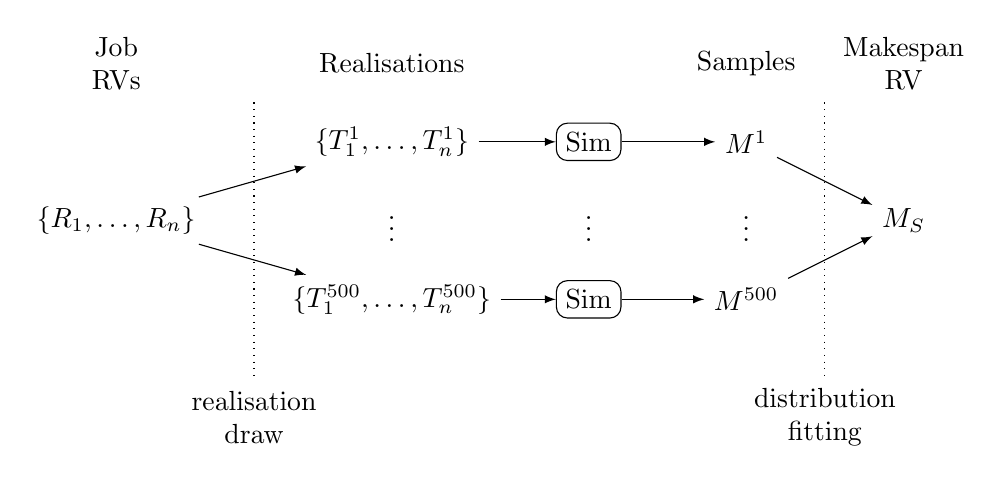
\begin{tikzpicture}[
sim/.style={%
draw, 
rounded corners
}
]
%% Origin node
\node[align=center]at(0,2){Job\\RVs};
\node at(0,0)(orig){$\{R_1,\ldots,R_n\}$};
%% Realisations
\node at(3.5,2){Realisations};
\node[]at(3.5,1)(pert1){$\{T_1^1,\ldots,T_n^1\}$};
\node at(3.5,0){\vdots};
\node at(3.5,-1)(pert5){$\{T_1^{500},\ldots,T_n^{500}\}$};
\draw[-{latex}](orig)--(pert1);
\draw[-{latex}](orig)--(pert5);
%%
\node[sim]at(6,1)(s1){Sim};
\node[sim]at(6,-1)(s5){Sim};
\node at(6,0){\vdots};
\draw[-{latex}](pert1)--(s1);
\draw[-{latex}](pert5)--(s5);
%% Makespans
\node at(8,2){Samples};
\node at(8,1)(M1){$M^1$};
\node at(8,-1)(M5){$M^{500}$};
\node at(8,-0){\vdots};
\draw[-{latex}](s1)--(M1);
\draw[-{latex}](s5)--(M5);
%% Consolidation
\node[align=center]at(10,2){Makespan\\RV};
\node at(10,0)(r){$M_S$};
\draw[-{latex}](M1)--(r);
\draw[-{latex}](M5)--(r);
%%phases
\node[align=center]at(1.75,-2.5)(df){realisation\\draw};
\draw[dotted](1.75,1.5)--(1.75,-2);
\node[align=center]at(9,-2.5)(df){distribution\\fitting};
\draw[dotted](9,1.5)--(9,-2);
\end{tikzpicture}

		}
\caption{Overview of a $500$-iteration Monte-Carlo simulation.}\label{fig:mc-process}
\end{figure}
The whole extended simulation process is referred to as \ac{mcs}. 
For an application composed of $n$ tasks (as depicted Fig.~\ref{fig:mc-process}),
\ac{mcs} consists in applying successive MCS-iterations. Assuming we can provide a
runtime distribution $T_j$ for every task $j$, a MCS-iteration $k$ consists in~:
\begin{itemize}
\item drawing a runtime value, $t_j$, for each task from the associated
	\acs{rv}, $T_j$;
\item proceed to a simulation using all runtimes $t_j$ to obtain a makespan $m_k$.
\end{itemize}
With enough  makespans $m_k$, we can  compute a statistical distribution  of the
makespan as a  final \ac{rv} noted $M$.  We extend our simulation  to two output
variables: we will not only observe the makespan computed at every iteration but
also the cost for each execution in number of \ac{btu}.


\subsection{Real Observations}
\begin{figure}[bt]
	\centering
	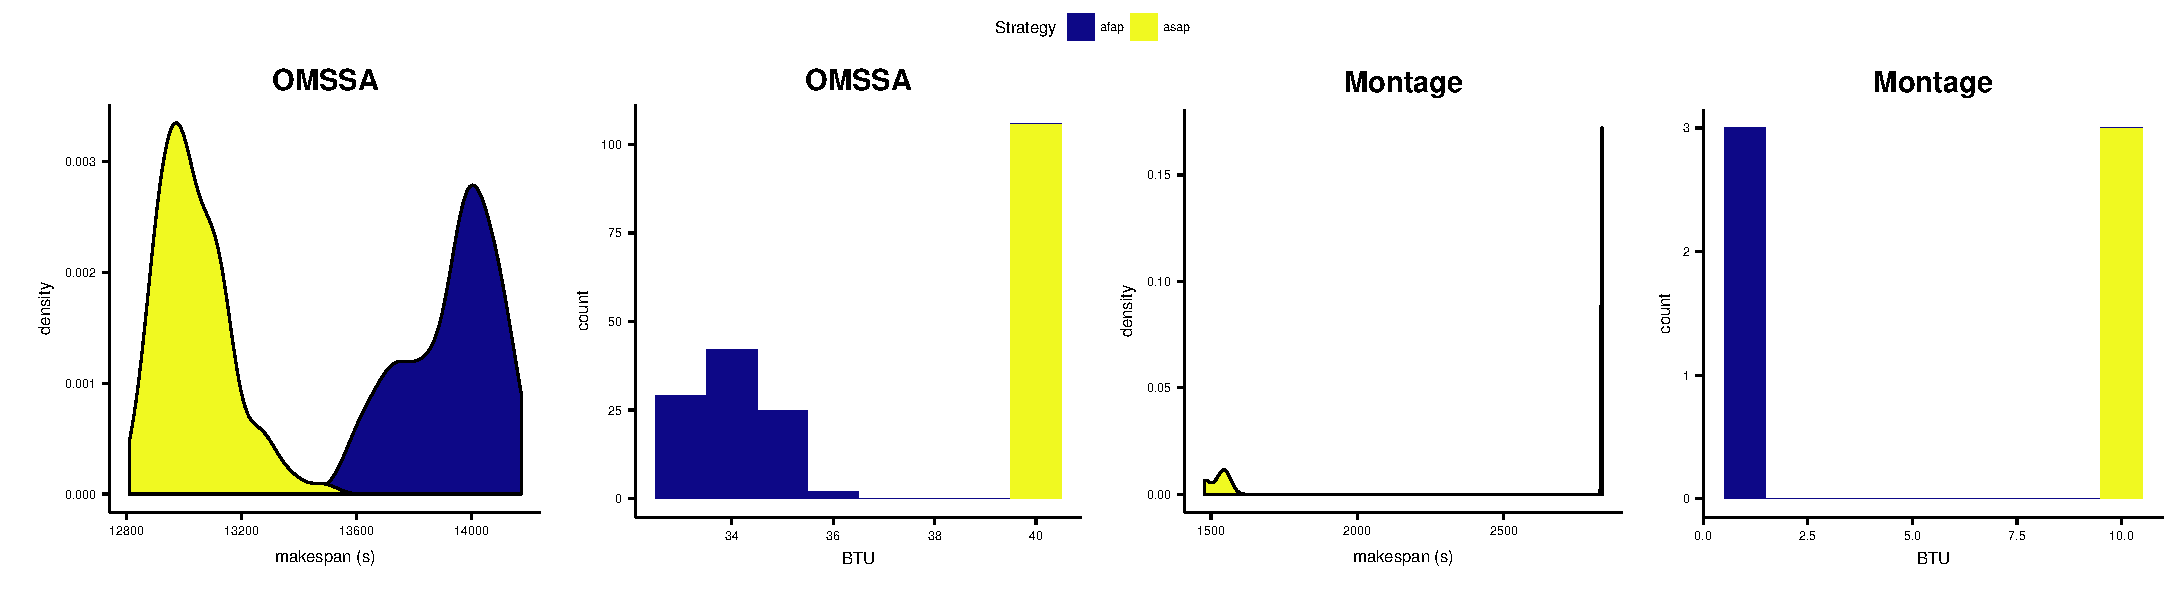
\includegraphics[width=\textwidth]{gfx/real_plot.pdf}
	\caption[caption]{Empirical observations for makespan distributions and \#BTU.%\\ 
	  %\textit{Reading example: Using AFAP with OMSSA leads to makespans 
	  %roughly ranging from 12800 s to 13600 s and BTU counts ranging from 33 to 36.}
	  }
	\label{fig:realbrs}
\end{figure}
\begin{comment}
\begin{table} \centering \caption{Overview of archived
	executions}\label{tab:nbruns} 
	\begin{tabular}{llrcc} \toprule
		Application&Strategy&\#runs&BTU count&Makespan ($s$)\\
		\midrule 
		\multirow{2}{*}{OMSSA}&ASAP&106&40&12811 -- 13488\\
				      &AFAP&98&33 -- 36&13564 -- 14172\\ 
		\midrule 
		\multirow{2}{*}{Montage}&ASAP&3&10&1478 -- 1554\\
				        &AFAP&3&1&2833 -- 2837\\
		\bottomrule 
	\end{tabular} 
\end{table}
\end{comment}

Using  Schlouder  (cf.  Section~\ref{sec:work-context}), we  performed  numerous
executions  of the  application  of  OMSSA and  Montage.  These executions  were
performed  on a  96 cores  Openstack cloud  system set  up on  4 identical  dual
$2.67GHz$ Intel  Xeon X5650 servers.  We used  the KVM hypervisor  and Openstack
version 2012.1  and 2014.4. The  traces obtained from these  experiments contain
several useful metrics  including, but not limited to, the  \ac{vm} start dates,
boot time, shutdown  times, and assigned tasks,  as well as the  task start date
and effective runtimes.
%
They were  initially used  all along  the development of  Schlouder and  then to
properly  tune SimSchlouder  in  order to  make the  simulation  as accurate  as
possible. As  a result, for the  execution used in this  paper, simulations done
with SimSchlouder are  precise to the second on the  makespan and systematically
exact on the \ac{btu} count.
%
Regarding variability, we find our platform variability to stand between 3\% and
6\% using the metrics described in the study~\cite{LeitnerC16} based on relative
standard  deviation of  tasks runtimes.   This variability  is within  the range
reported in  the study for platforms  like Amazon's EC2 or  Google Cloud Engine,
with the exception of shared CPU instances.

In this  paper these execution  traces are used  to generate our  \ac{mcs} input
\acp{rv}  using the  method  we  will describe  in  Section~\ref{sec:im} and  we
compare  the  makespan  and  \ac{btu}  distributions  of  the  \ac{mcs}  to  the
distribution observed in the corresponding traces. For this purpose, traces from
comparable runs are grouped by application and strategy.  Fig.~\ref{fig:realbrs}
presents  the distribution  of  resulting makespans  and  \ac{btu} counts.   For
OMSSA,  ASAP   yields  a  makespan   variation  in  the   range  [12811s;13488s]
(variability $\approx$5\%)  with a  constant BTU  count of  40, and  AFAP yields
[13564s;14172s]  (4\%)  with a  BTU  count  ranging  [33;36]. For  Montage,  the
makespans are in  the range [1478s;1554s] ($\approx$ 4\%) with  10 BTUs for ASAP
and [2833s;2837s] (0.1\%) with 1 BTU for AFAP.


\subsection{Input Modeling}\label{sec:im}


Using a  \ac{mcs} we can account for this  variability and provide the
user with  a range of  possible makespans. In this  section we propose  a simple
model to  represent the variability of  the whole system using a single factor
parameter to create  a small range around every estimated  runtime. We test this % ne pas mélanger modele/approche et valdiation
model against our backlog of real runs. The key finding detailed hereafter is
that this simple model can be precise enough for the  \ac{mcs} to predict over
90\% of real runs.

This model for the runtimes \acp{rv} uses uniform distributions ($\mathcal{U}$). 
These \acp{rv} are centered on the estimated runtime of the task they represent.
The relative spread of these distributions is defined by the \emph{perturbation
level} $P$, which is the same for every task.  If we assume $P$ can summarize
the variability of the whole system, a central question is how should $P$ and
the user estimates be chosen to assess the validity of the \ac{mcs}. To this
end, we assume a good guess for an  estimated runtime is the  average of all
effective runtimes, $\bar{r_j}$ for a given task $j$. As such the runtime
distribution's \ac{rv} $T_j$ for task $j$ is: 
\begin{equation} 
	T_j = \mathcal{U}(\bar{r_j}\times(1-P), \bar{r_j}\times(1+P))
\end{equation}

Since the global perturbation level $P$ establishes the limit for the worst
deviations from the estimated runtimes, the relative standard deviation metric
used in~\cite{LeitnerC16} is not well suited. Instead we choose to build $P$
using the average of the worst observed deviation for every task in the
application. With $r_j^n$ the $n$th runtime observation for task $j$, $P$ is set
to~:

\begin{equation}
	P =
	\underset{j}{\textrm{mean}}\left(\max_n\left(\frac{|r_j^n-\bar{r_j}|}
	{\bar{r_j}}\right)\right)
\end{equation}

For OMSSA, the perturbation level given by this model is $P\approx{}10\%$ for both
strategies. For Montage  our calculated perturbation level is  $P\approx{}20\%$
for ASAP and $P\approx{}5\%$ for AFAP. Using a similar metric, \cite{pics} also 
observed most deviations to be within 10\% of the average runtime when working on
Amazon EC2 instances with dedicated CPUs.

\section{Evaluation}
\label{sec:eval}
\begin{figure}[bt]
	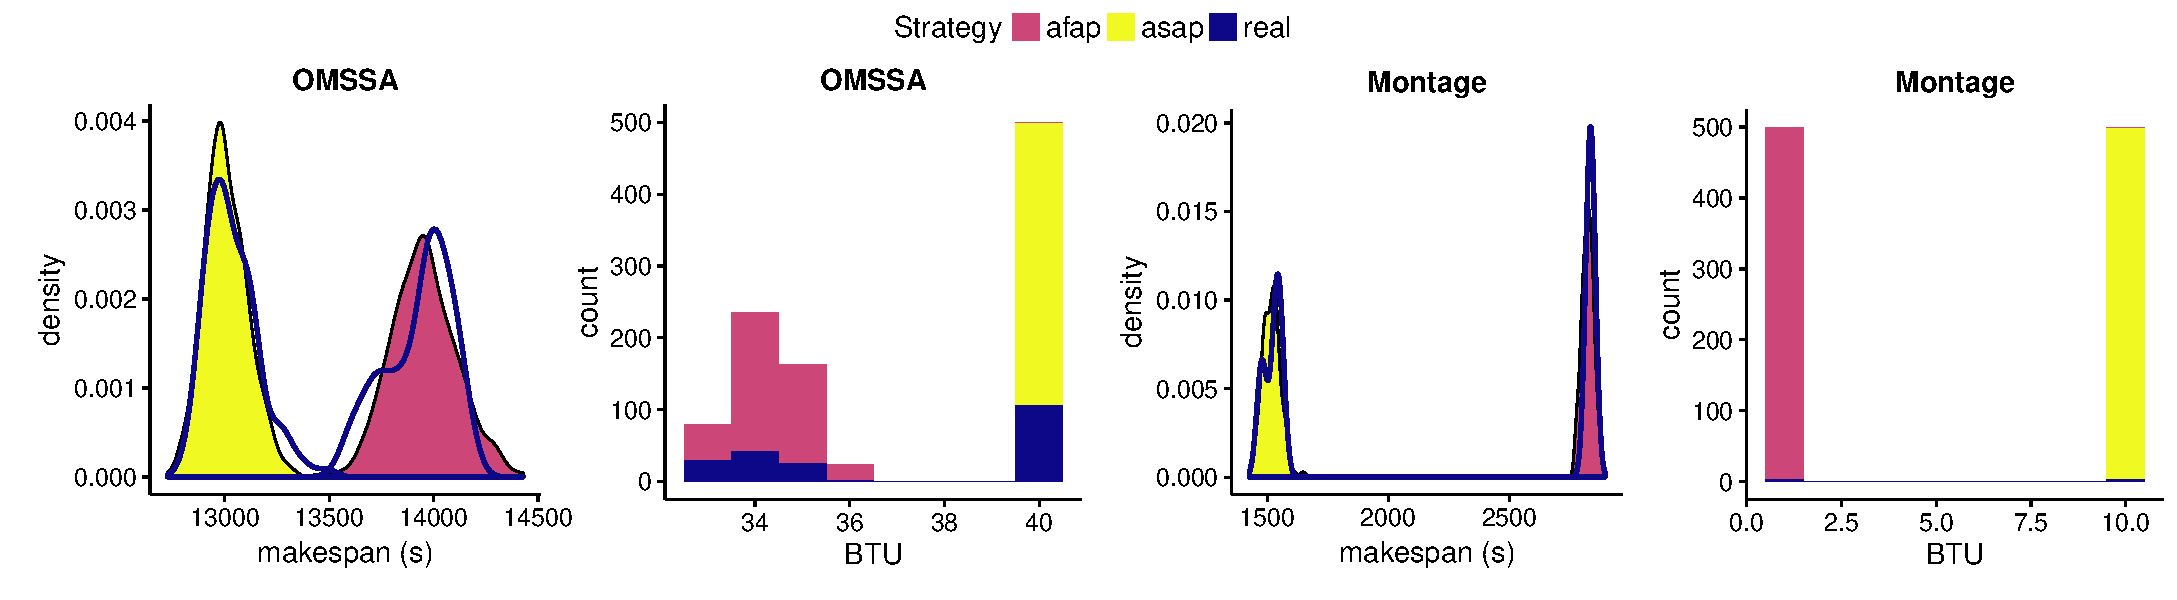
\includegraphics[width=\textwidth]{gfx/fit_plot.pdf}
	\caption[caption]{Makespan and \#BTU distributions for MCS compared to
		reality for $P=10\%$.%\\ 
	  %\textit{Reading example: Simulating AFAP with OMSSA leads to makespans 
	  %roughly ranging from 12800 s to 13400 s and BTU counts ranging from 33 to 36.}
	}
	\label{fig:fit}
\end{figure}
We ran a 500-iteration \ac{mcs} for every strategy application group using
the task model described in  the previous section. The  resulting distributions
are  shown  in  Fig.~\ref{fig:fit}.   The makespan  density  graphs  show  the
simulation  result  distribution   as  filled  curves. The  real  observed
executions, as in  Fig.~\ref{fig:realbrs}, are shown as  non-filled curves. On 
the \ac{btu} count graphs, the  left bar represents
the empirical data, and the right  bar the results from the simulation.
%
These graph show the simulation results cover the same ranges as the real
observation, but do not present the same distribution within those ranges. 
%
%When looking at the resulting OMSSA distributions, presented in the two leftmost
%graphs,  the distribution  of simulated  makespan ranges  covers fairly  well the
%ranges of  observed makespans, notwithstanding a  slight right skew and  shift of
%the empirical  makespan distribution.  The  OMSSA BTU count  distributions shows
%similar results.  The range of BTU  numbers required for an execution is correct.
%For instance,  both empirical  observations  and simulations  indicate
%between  33 and  36 BTU  are used with AFAP. However, the  distributions of  these BTU  counts
%differ slightly.
%
We quantify our simulation results correctness using statistical confidence
intervals.   Since the makespan is in essence  the sum of the tasks' runtimes
in the  execution critical path,  and tasks  are all distributed  using the
uniform distribution  which  has a  finite variance,  we consider the Central
Limit Theorem applicable.  Fitting to a normal distribution gives us an average
makespan $\mu{}$, and a standard deviation $\sigma{}$. These can be used to
build \acp{ci}. For the normal distribution  the 95\% \ac{ci}, defined  as
$[\mu{}-2\sigma{},\mu{}+2\sigma{}]$  and   the  99\%   \ac{ci},
$[\mu{}-3\sigma{},\mu{}+3\sigma{}]$.
%
\begin{table}[b]
	\centering
	\caption{Makespan and BTU capture rate depending on CI
          for P=10\%.}
       \label{tab:fit} 
	\begin{tabular}{llccc}
		\toprule
		Application&Strategy~&\multicolumn{2}{c}{~Makespan (Size of
		CI)~}&~BTU\\
                           &         & CI 95\% & CI 99\% &\\
		\midrule
		\multirow{2}{*}{OMSSA}&ASAP&  90\% (3\%)&  98\% (5\%)& 100\%\\
				      &AFAP&  92\% (4\%)& 100\% (6\%)& 100\%\\
		\midrule
		\multirow{2}{*}{Montage}&ASAP& 100\% (2\%)& 100\% (4\%)& 100\%\\
					&AFAP& 100\% (1\%)& 100\% (2\%)& 100\%\\
		\bottomrule
	\end{tabular}
\end{table}
%
The capture rate expresses the number of observed real makespans that fall
within a given \ac{ci} relative to the total number of real observations.
Table~\ref{tab:fit} presents the capture rate obtained by each interval computed
after normal fitting.  Additionally we provide for each interval its size
relative to the average makespan.
%
Regarding OMSSA, the \ac{mcs} captures at least 90\% of real observed
makespans. The divergence between the capture rate and the \ac{ci} expected
capture  rate is due  to the fact that the  empirical makespan distribution does
not follow a perfect normal distribution. Using  a 99\% \ac{ci} improves the
capture  rate up to  98\%, hence very close to the theoretical expectation.
Regarding Montage the \ac{mcs} achieves a capture rate of 100\% for any
\ac{ci}.


Our \ac{mcs} and a simple task model can capture 90\% of reality all the while
producing makespan intervals of limited size, a 3\% relative size representing 7
minutes on a 3h 45m long makespan. We consider this result a satisfactory
trade-off between the simplicity of the input model and the accuracy with
regards to the theoretical \ac{ci}.


\section{Perspectives}
\label{sec:disc}
Outside of the realm of reproduction or predictions, we believe that \ac{mcs}
can have other more research oriented applications. In this section we will
exemplify one such application. Then we will discuss limitations we have
encountered in our work with \ac{mcs}.

\paragraph{High perturbation simulations.}\label{sec:sa}
\begin{figure}[bt]
	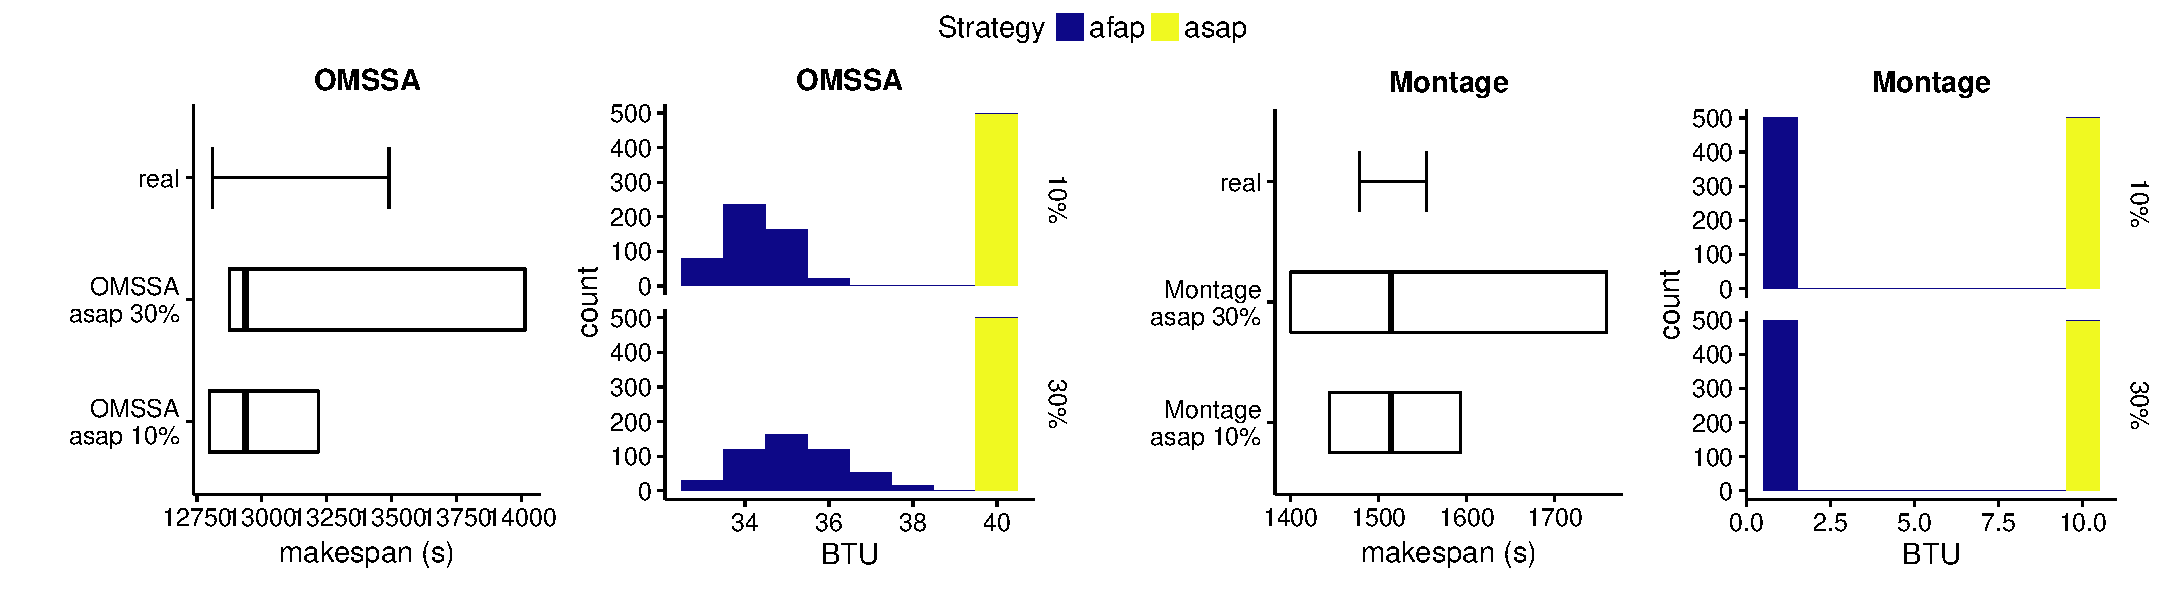
\includegraphics[width=\textwidth]{gfx/int_plot.pdf}
	\caption[caption]{Makespan intervals and \#BTU distributions for OMSSA and 
	Montage at different perturbation levels. In the makespan interval graph 
	the boxes represent the 95\% CI resulting from the normal fit of the
	\acs{mcs}'s results, and the bar the results of a single unperturbed 
	simulation.%\\
	%\textit{Reading example: Using ASAP and the runtimes from one real OMSSA
	%run having a makespan of 13000 s, the simulations with a perturbation 
	%level of 10\% leads to makespans roughly ranging from 12800 s to 13250 s, 
	%while the makespans from the complete set of real runs range from 12800 s to 13500s.}
	}
	\label{fig:int}
\end{figure}
We have so  far set the perturbation level  to a value that was  relevant to the
real system observed  (see Section~\ref{sec:im}).  A subsequent  question is how
does the  prediction change  when increasing this  perturbation level.   In this
section  we will  focus  on simulation  of makespans  using  the ASAP  strategy.
Fig.~\ref{fig:int}  presents  the  95\%  \acp{ci} obtained  through  the  normal
distribution fitting of  simulations with both $P\!=\!10\%$ and $P\!=\!40\%$.  Notice that a
40\% perturbation level may be experienced in current cloud provider offers when
renting shared  instances (\cite{LeitnerC16}).  On the  makespan interval graphs
(first and third subfigures from left to  right) the boxes represent the span of
the \ac{ci}  interval. The mean  simulated makespan ($\mu{}$) is  represented by
the vertical bar inside the interval. The middle row shows the interval of real 
observed makespans.
%
Simulation of OMSSA using $P\!=\!40\%$ exhibits a clear drift upward of
the ranges of simulated makespans and BTU. This drift is significant compared to
the growth of the capture interval to the point that the capture rate of the
simulation with $P\!=\!40\%$ is of only 83\% when the $P\!=\!10\%$ simulation had a 90\% 
capture rate. Montage simulations exhibit the upwards drift but not to the
extent that it affects the simulation's capture rate. These results have two 
interesting implications.
%
%The leftmost subfigure presents the \acp{ci} for the \{OMSSA, ASAP\} group at
%40\% and 10\% perturbation levels. With the increase of the perturbation level
%the intervals naturally get wider, but the average makespan also increases. 
%This happens to the 
%extent that the lower bound of our interval at 40\% is higher than the lower
%bound at 10\%. This diminishes the capture rate of the simulation from 90\%
%(table~\ref{tab:fit}) to 83\% even as the relative width of the interval grows
%from 3\% (7 minutes) to 10\% (almost 24 minutes). For \{Montage, ASAP\} we observe
%again an increase of the average makespan, but not as much as the increase in
%the \ac{ci}'s width. Therefore the \ac{ci} resulting from the \ac{mcs} at a
%40\% perturbation level is a superset of the one at 10\% perturbation level.
%These results have two interesting implications.
%
Firstly, the perturbation level can
not be used as a trade-off variable to augment capture rate at the expense of
\ac{ci} compactness. The lower capture rate at $P\!=\!40\%$ is a
strong indication that our real platform exhibits a variability closer to
10\% than to 40\%. Misestimation of the perturbation level will have the same
implication for the \ac{mcs} as a wrong effective runtime given to \ac{des}. 
Users for whom higher capture rates are more important than
interval compactness should use statistical methods to build higher rate \acp{ci},
like the 99\% normal distribution \ac{ci} used in section~\ref{sec:eval}.
%
Secondly, this result shows that \ac{mcs}s can be used to exhibit strategy
behaviours. This upwards shift of the \ac{ci} shows that ASAP, a strategy
geared towards reducing the makespan regardless of cost, is not as effective
when scheduling bag-of-tasks with task runtimes that might vary widely. However,
the same observation on Montage shows that when scheduling workflows ASAP 
remains capable of low makespans. This behaviour is explained by the nature of 
workflows, in which tasks have to wait for their latest dependencies resolution 
to run. In workflows the makespan depends only on the execution critical path, 
and are therefore unaffected by the variability of tasks outside the path. 
This kind of analysis can be used to gain insight in the strengths and 
weaknesses of any strategy, regardless of complexity.

\paragraph{Limitations of the enriched simulation.}\label{sec:lim}
%
In this paper  all the \ac{mcs} presented used 500 iterations. Such an \ac{mcs}
requires in average 15 minutes of  CPU time, and iterations can be parallelized.
We  determined  that  this was  enough  in  the  context  of our  simulation  as
additional simulations did not change  the results and only marginally increased
the confidence of the fitting process. The number of simulations necessary in an
\ac{mcs} depends on the number of  input variables and the distribution of these
variables.   A \ac{mcs}  works  by  sampling the  possible  scenarios  to get  a
distribution of possible  outcomes, hence when more scenarios  are possible then
more samples are required.  The relative quick convergence (as compared to other
scientific fields  where \ac{MCS} is  used) is  explained by the  relatively low
number of input variables found in batch job scheduling.  In our case, there are
respectively 223 and 184 tasks for  OMSSA and Montage. As the perturbation level
influences the  input variable distribution,  we are currently studying  how its
relationship with the number of required MCS-iteration.

\section{Conclusion}
Predicting  the execution  behaviour of complex  workloads in  the  cloud is  an
important challenge. While a number of research works have proposed model-driven
simulators, much remains to be done for their adoption in production-grade cloud
settings. As  advocated by Puchert  et al.~\cite{PucherGWK15}, the trust  we can
put in  the prediction  demands certainty  and precision  that only  comes from
validating simulation against empirical observation.
%
This paper contributes to this effort in two ways. First, we propose a \acl{mcs}
extension  to a  discrete  event  simulator based  on  SimGrid.  This  extension
provides stochastic predictions which are more informative than single values of
billing cost  and makespan  produced by  traditional discrete  event simulators.
The \acl{mcs}  must be parameterized to  draw random values from  relevant value
spaces. In this work we show that the  variability we seek to account for can be
modeled  by a  single parameter,  called perturbation  level and applied  to all
task runtimes. Second, we apply our model in  a real setting, on both a
bag-of-tasks and a workflow  application, for which we have collected  execution
traces, using scheduling and provisioning strategies that  aim to optimize
either the makespan or the  rental cost.  At  the light of  these empirical
observations,  our study shows that the proposed model could capture over 90\%
of the observed makespans for  all  combinations  of  application   and
scheduling  strategies  given  an appropriate perturbation  level. We now aim
to test our simulator  on more use cases and platforms.  In particular as a
number of studies on public clouds have reported variability levels similar to
our platform (\cite{LeitnerC16,pics}), we intend to reproduce these results on
public clouds.

\bibliographystyle{splncs}
\bibliography{montecarlo-simulation}

\end{document}
% vim:spell spelllang=en:
